\documentclass[12pt,a4paper,titlepage,oneside]{article}
\usepackage[utf8]{inputenc} 
\usepackage[T1]{fontenc}
\usepackage{protocol}
\usepackage{listings}
\usepackage[T1]{fontenc}
\usepackage{times}
\usepackage{epsfig}
\usepackage{epstopdf}
\usepackage[german, english]{babel}
\usepackage{listings}
\usepackage{textcomp}
%\usepackage[normalem]{ulem}
\usepackage{tabularx}
\usepackage{amssymb,amsmath}
\usepackage{color}
%\usepackage{framed}
\usepackage{makeidx}
\usepackage{natbib}
\usepackage{textcomp}
\usepackage{alltt}
\usepackage{array}
\usepackage{rotating}
\usepackage{lscape}
\usepackage{graphicx}
\usepackage{import}
\usepackage[bookmarks]{hyperref}


\usepackage{verbatim}


%%%%%%%%%%%%%%%%%%%%%%%%%%%%%%%%%%%%%%%%%%%%%%%%%%%%%%%%%%%%%%%%%%%%%%%%%%%%%%%%%%%%%%%
% Alter some LaTeX defaults for better treatment of figures:
    % See p.105 of "TeX Unbound" for suggested values.
    % See pp. 199-200 of Lamport's "LaTeX" book for details.
    %   General parameters, for ALL pages:
    \renewcommand{\topfraction}{0.9}	% max fraction of floats at top
    \renewcommand{\bottomfraction}{0.8}	% max fraction of floats at bottom
    %   Parameters for TEXT pages (not float pages):
    \setcounter{topnumber}{2}
    \setcounter{bottomnumber}{2}
    \setcounter{totalnumber}{4}     % 2 may work better
    \setcounter{dbltopnumber}{2}    % for 2-column pages
    \renewcommand{\dbltopfraction}{0.9}	% fit big float above 2-col. text
    \renewcommand{\textfraction}{0.07}	% allow minimal text w. figs
    %   Parameters for FLOAT pages (not text pages):
    \renewcommand{\floatpagefraction}{0.7}	% require fuller float pages
	% N.B.: floatpagefraction MUST be less than topfraction !!
    \renewcommand{\dblfloatpagefraction}{0.7}	% require fuller float pages

	% remember to use [htp] or [htpb] for placement
%%%%%%%%%%%%%%%%%%%%%%%%%%%%%%%%%%%%%%%%%%%%%%%%%%%%%%%%%%%%%%%%%%%%%%%%%%%%%%%%%%%%%%%

%"C:\Program Files\MiKTeX 2.9\miktex\bin\pdflatex.exe" main.tex


\lstset{
  backgroundcolor=\color{lbcolor},
  tabsize=4,
  rulecolor=,
  language=C, %VHDL
  basicstyle=\scriptsize,
  upquote=true,
  aboveskip={1.0\baselineskip},
  columns=fixed,
  showstringspaces=true,
  extendedchars=true,
  breaklines=true,
  prebreak = \raisebox{0ex}[0ex][0ex]{\ensuremath{\hookleftarrow}},
  frame=single,
  showtabs=false,
  showspaces=false,
  showstringspaces=false,
  identifierstyle=\ttfamily,
  keywordstyle=\color[rgb]{0,0,1}\ttfamily,
  commentstyle=\color[rgqb]{0.133,0.545,0.133}\ttfamily,
  stringstyle=\color[rgb]{0.627,0.126,0.941},
  numberstyle=\colr{black}\ttfamily,
}
\definecolor{listinggray}{gray}{0.9}
\definecolor{lbcolor}{rgb}{0.97,0.97,0.97} %gray
%\definecolor{lbcolor}{rgb}{1.0,1.0,1.0} %white



\definecolor{myyellow}{rgb}{1.0,1.0,0}
\definecolor{mygray}{rgb}{0.5,0.5,0.5}
\definecolor{mylime}{rgb}{0.6,1.0,0.2}
\definecolor{mycyan}{rgb}{0.0,1.0,1.0}



\definecolor{green}{RGB}{0,255,0}

\sloppy

\exercise{
  {\huge Network Embedded Systems [VU]} 
  \par
  {\huge Semster Project - Protocol}
  \par
}
% fancy projektname fehlt noch..wem fällt was ein??

\authors{
  Helmut Bergmann, Matr.Nr. 0325535  \par
  {\small 0325535@student.tuwien.ac.at} \par
  Bernhard Fritz, Matr.Nr. 0828317  \par
  {\small 0828317@student.tuwien.ac.at} \par
  Marko Stanisic, Matr.Nr. 0325230 \par
  {\small 0325230@student.tuwien.ac.at} \par
}


\begin{document}

\maketitle
%\tableofcontents
%\clearpage

\pdfinfo{
   /Title  (Sensor Testing 1 - Protocol)
   /CreationDate (\today)
%   /Subject ()
%   /Keywords ()
}


%\cite{sharc_hw_ref}
%\cite{sharc_prog_ref}
%\cite{ezkit_manual}
 
 
%-----------------------------------------------------------------------------
%   content
%-----------------------------------------------------------------------------
 
\section{Requirements}
% Introduction about the project etc...

The requirements come here..

It should water the flowers...
\begin{itemize}
\item Reliable flower watering
\item It should be quiet
\item An efficient solution
\item The hardware solution should be visually appealing
\item Data should be logged to perform statistical analysis on it.
\item The data connection should be wirelessly
\end{itemize}


\section{Design}
The network infrastructure consist of a IOT controller, a data logger, sensor nodes and pump nodes.


\subsection{Sensor Node}
%about the sensor node...

The sensor node provides the current state of the flower environment to the controller.
It is a low power device which guarantees long battery duration.

The sensors used are:
\begin{itemize}

\item Temperature sensor
It shows the temperature...

\item The second sensor is a moisture sensor. It consists of two parts, a resistance probe (YL-69) and a control board (YL-38). The probe will be put into the measured soil, while the board should stay dry. The Arduino nano has a 10 bit ADC, so the result read from the ADC is an integer between 0 and 1023.\\


The test showed that in a dry state the sensor shows 1023. Connecting the electrodes with a finger leads to a value around 1000.\\
Also in dry soil the readout is 1023, but as we pour water into the pot, it continuously decreases down to a few hundred. (I did not want to drown the flower, but I assume it goes to 0 if we put the probe into water...)\\

We might have to calibrate the moisture levels for different flower or soil types, but in general the sensor seems to do the job very well and also is usable with a XBee board because of its analog output. The only downside is that it's written in forums that after some weeks this type of sensor will be corroded, so we cleaned it as well as possible after the test. For developing and testing it is fine, in a real environment one might want to use another sensor like a capacitive one or with other electrode materials. Also turning off the sensor when not using it is a good approach to avoid this problem.\\
% Man könnt hier noch einen konkreten Sensorvorschlag machen, der auch mit ADC funktioniert 

\item
The last sensor to test was a photoresistor which is a semiconductor that reacts to light. It was also provided in the Arduino kit. The manual suggested the range of the photoresistor is between 500$\Omega$ (bright) and 50$k\Omega$ (dark). 
Further it suggested to use a 1$k\Omega$ resistor for the voltage divider. An arduino tutorial \citep{misc:photoresistor_tutorial} suggested 10 $k\Omega$. So we decided to measure the actual resistor values and use the formula from the lecture to calculate the matching resistor of the voltage divider. % , 26$k\Omega$ was a good choice  

The measurements showed that the actual photoresistor range is 500$\Omega$ to 1.7$M\Omega$.\\
\begin{equation}
R_1 = \sqrt{R_{max}*R_{max}} = \sqrt{500*1700000} = \sqrt{850000000} = 29k\Omega
\end{equation}


The closest resistor available to us was 26$k\Omega$.\\
These values differ to those suggested by the tutorials, but since also the photoresistor has different values, our choice seems feasible. Also we are convinced a higher resistor will not harm the components in contrast to a low resistor.\\
So we connected the chosen pulldown resistor between ground and the A1 pin of the Arduino Nano. To complete the voltage divider the photoresistor was connected between VCC and the A1 pin.\\

Sketches again are provided by online tutorials and the Arduino kit producer. Although it is very similar to the one for the moisture sensor, just another pin is used.\\

The test worked very well, close to a light bulb we get values over 950 and if we cover the photoresistor it drops to under 30. That confirmed our choice of the resistor.\\

We can conclude that this sensor is easy to work with and compatible with XBee, as no special protocols are required.

\end{itemize}



\subsection{Controller}
The controller keeps track of all nodes and handles their registration.
It executes the watering policy that the user has selected for each flower.
For this task it wirelessly communicates with the sensor node situated in the flower pot and the pump node situated next to the water tank. The sensor node provides the controller with the most recent measurement values, whereas the pump node executes the pump commands received from the controller.

\subsubsection{State diagram}

\begin{figure}[h!]
	\begin{center}
	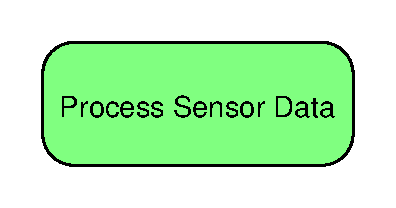
\includegraphics[scale=0.24]{../ControlNode_Diagramm.pdf}
	\caption{Overview of the chosen setup.}
	\label{Setup_overview}
	\end{center}
\end{figure}


States:
\begin{itemize}
	\item Check pending tasks

		This is the begin of the loop() Function. The controller will always come back to this state to check which tasks are pending. The following actions are possible:

		\begin{itemize}
			\item A NRF24 message is arrived, process this message.
			\item Also if an interactive command has arrived via the IOT framework, this command has to be processed. (Typically sending an instruction to a Motor Node)
			\item If, according to the watering schedule, a pump node should take an action now, the controller goes to the ``Send Watering Command to Motor Node'' state
			\item If a Motor Node did not respond as expected, an error handling sequence should be started (writing to log and if needed respond to the IOT framework)
		\end{itemize}

	\item Send Watering Command to Motor Node
		Whenever the controller decides a pump node should start to pump, this function is called. 			It prepares and sends a message to concerned the pump node. It also writes the message content to a log file.
	\item Write Pump Node Timeout to Log
		If a pump node does not reply within the specified timeout duration, an entry into the log file has to be written. In case the command of the concerned message has been triggered by the IOT framework, the controller will move to the ``Send Error Notification to App'' state. Otherwise it enters the ``Reschedule Watering'' state.
	\item Send Error Notification to App
			If a IOT command could not be successfully executed, the IOT framework has to be notified about the problem. Afterwards the controller goes back to checking for pending tasks.
	\item Reschedule Watering
		If a scheduled watering task failed, the controller needs to reschedule this watering task.
		There are many possible algorithms for this such as:
		\begin{itemize}
			\item Skip this watering task and proceed as usual
			\item Retry the watering task a certain number of times. If it fails, proceed as usual
			\item Reschedule the watering of this pump node in a given fashion.
		\end{itemize}
		For a first version it is sufficient to skip the watering, if it failed.
		
	\item Write Motor Node Response to Log File
		If a motor node responds to a control command, this response has to be logged to a log file. Afterwards the controller processes the response.
	\item Mark Command as Read
		The watering command is marked in the controller internal command list as ``read by the node''. Otherwise a timeout would occur.
		
	\item Process State Message
		As the pump node finished to pump, it will send a state message to the controller indicating the end of the pump sequence. This message can be responded to by the controller, but it doesn't have to be.
		
	\item Process Sensor Data
		When the controller receives data from a sensor node, it stores the data. Later this data will be used for the watering algorithm and statistical analysis. Afterwards it will check whether the sensor node has data stored in its EEPROM. This will be the case if the controller was unavailable to the sensor node for some time. If there is EEPROM data the controller can choose whether it wants the data to be transmitted now, later or not at all. If the latter is the case, the node will delete its sensor data. If the controller has currently time to receive the EEPROM data, it should request it. Otherwise the data might get lost. If there is a lot of traffic scheduled in the next slots, the controller can postpone the EEPROM data transmission. In this case the next sensor node transmission should be scheduled in a slot that is followed by empty slots. This way it is guaranteed that there is enough time to transmit all EEPROM data.
	
	\item Respond
		In the respond state a response is prepared and sent to the node from which the last message has been received. Its content is based on the previous states.
		
	
	
\end{itemize}


\subsection{Pump Node}


\subsubsection{Fall-back Mode}
To guarantee a dependable solution resistant to external factors such as a failing internet connection or wireless jamming attacks, a fall-back mode has been implemented to water the flowers reliably, even if the control node is unavailable.

For this purpose the pump node uses all incoming messages, also those addressed to other nodes, to detect the availability of the controller. If the pump node does not receive any messages from the controller for a specified timeout\_duration, it assumes the controller is offline and goes into a fall-back mode.

The parameters for the fall-back mode are:
\begin{itemize}
\item timeout\_duration
\item enable
\item time
\item watering\_duration
\end{itemize}

These parameters can be set at the IOT front-end-interface and get transmitted to the pump nodes by the controller at the pump node registration and with every pump request. (so in case they get changed the pump node stays up to date)
In case the fall-back is disabled, no action takes place if the controller is unavailable.
In case the fall-back is enabled and the controller is unavailable, daily at the specified time the pump node pumps for the specified watering\_duration.

This mechanism does not guarantee a perfect watering, however it prevents the plants from drying.

To make the fall-back visible to the monitor node, a notification message is broadcasted via the wireless network containing the timestamp, pump duration and last timestamp from a controller message.


\subsection{Protocol}
For registering nodes and perform data exchanges a protocol has been developed. The developed library provides access to the protocol registers to use the functionality of the protocol.


Status register in the node --> controller message:

\begin{table}[htbp]
        \small
        \setlength\tabcolsep{2pt}
\begin{tabular}{ l c c c c c c r }
%  Test ID & measurement base frequency [MHz] & measurement scale factor & PLL factors (m/d) & measurement frequency [MHz] & PISO base frequency [MHz] & PISO scale factor & PISO frequency [MHz]\\ \hline
  Bit & name & description & 0 - meaning & 1 - meaning\\ \hline
  0 & RTC\_RUNNING\_BIT & RTC is paired on the node & no RTC & RTC paired \\ \hline
  1 & MSG\_TYPE\_BIT & type of message & registration request & data \\ \hline
  2 & NEW\_NODE\_BIT & new or known node & known node & new node \\ \hline
  3 & EEPROM\_DATA\_AVAILABLE & is data in the EEPROM & no data & data available\\ \hline
  4 & EEPROM\_DATA\_PACKED & kind of data & live data & EEPROM data\\ \hline
  5 & EEPROM\_DATA\_LAST & more EEPROM data pending & more data & not more data \\ \hline
  6 & NODE\_TYPE & type of node & sensor node & pump node\\ \hline
\end{tabular}\\
\end{table}


Status register in the controller --> node message:


\begin{table}[htbp]
        \small
        \setlength\tabcolsep{2pt}
\begin{tabular}{ l c c c c c c r }
%  Test ID & measurement base frequency [MHz] & measurement scale factor & PLL factors (m/d) & measurement frequency [MHz] & PISO base frequency [MHz] & PISO scale factor & PISO frequency [MHz]\\ \hline
  Bit & name & description & 0 - meaning & 1 - meaning\\ \hline
  0 & REGISTER\_ACK\_BIT & registration acknowledge & no reg & registration\\ \hline
  1 & FETCH\_EEPROM\_DATA1 & &  &  \\ \hline
  2 & FETCH\_EEPROM\_DATA2 &  & &  \\ \hline
  3 & ID\_INEXISTENT & id invalid & id valid & id invalid\\ \hline
\end{tabular}\\
\end{table}

Further the combination ``00'' in the FETCH\_EEPROM\_DATA1/2 bits indicates the EEPROM data shouldn't be transmitted now, ``01'' means the sensor node should send the data now and ``10'' means the node should delete the stored EEPROM data.



%-----------------------------------------------------------------------------
%   bibliography
%-----------------------------------------------------------------------------

\clearpage 
\phantomsection
\addcontentsline{toc}{section}{References}
\bibliographystyle{plain}
\bibliography{references}
\printindex
\printindex

\end{document}

